
    \begin{abstract_online}{Topological Identification Criteria, Stability and Relevance of Pentagonal Nanochannel in Amorphous Ice }{%
        \underline{N. Pingua}, P. A. Apte}{%
        }{%
        Department of Chemical Engineering, IIT Kanpur, India}
    The fivefold symmetric structure is commonly found in nature [1] and in different class of materials such as metallic glasses, [2] metal-alloys, [3] nanocrystalline materials, [4] and hard-sphere systems, [5]. Considering the potential importance of pentagonal nanochannels (PNCs) in determining the structure of the amorphous ice, we introduce topological criteria to identify the PNCs with an optimal fivefold symmetric environment. The basic building block in our criteria (see Figure1), termed as a bicyclo octamer, is an axisymmetric cluster formed by combination of three six-membered boat-shaped rings. The shape of boat and chair rings identify using dihedral angle criteria. [6] This bicyclo octamer unit serves as a seamless interface of the PNCs with cubic-hexagonal stacking patterns of the amorphous ice. This interface results in a fivefold symmetric mesostructure of relatively high stability: a central PNC with extended five branches of two-dimensional (2-D) hexagonal (wurtzite) crystalline monolayers stacked with cubic (diamond) layers. We also unearth a hierarchy of symmetric structures in amorphous ice: the PNCs, together with dodecahedron cages, form a network consisting of (nearly) equilateral triangular patterns. At the next hierarchical level of symmetry, such triangular patterns combine to form triangular pyramids with dodecahedron cages as the vertices, PNCs as the edges, and confined 2-D hexagonal crystalline monolayers as the triangular faces of the pyramids. The central core of the pyramids consists of cubic (diamond) regions with a strong local tetrahedral order. The overall structure of the amorphous ice states is found to be profoundly affected by PNCs. Specifically, in states with a relatively large number of PNCs, the cubic- hexagonal stacking is primarily in the form of hexagonal crystalline monolayers stacked from both sides with cubic crystalline layers [7]. \begin{center}  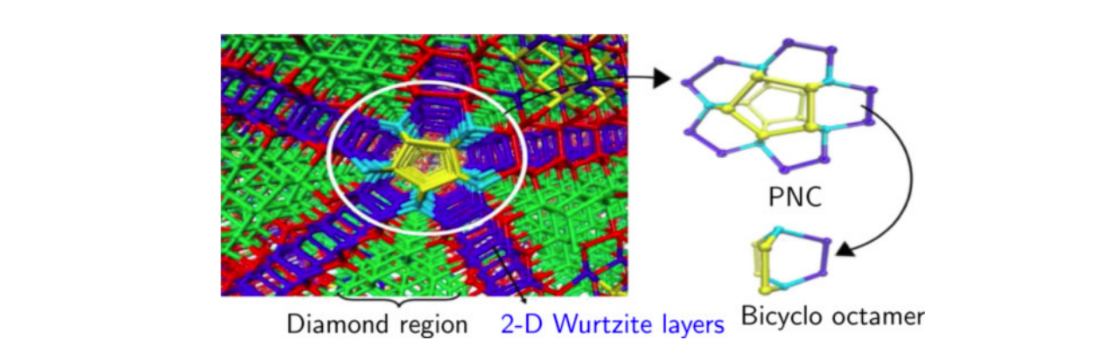
\includegraphics[width=\linewidth]{abstracts/txt/figures/nandlal.png}  \caption{\textbf{Figure 1:} Basic building block to identify the pentagonal nanochannel (PNC).}  \end{center} 
    
        \textbf{References} \newline{}[1] I. Hargittai, Fivefold symmetry, World scientific: Sinapore (1992)\newline{}[2] Y. Q. Cheng and E. Ma, Prog. Mater. Sci., 56, 379-473, (2011)\newline{}[3] C. Y. Hu, X. F. Li, Z. M. Li, Y. H. Bai, and H. W. Wang, Nat. Commun. 6, 8310, (2011)\newline{}[4] C. J. Johnston, and V. Molinero, J. Am. Chem. Soc. 134, 6650-6659, (2012)\newline{}[5] B. O’Malley, and B. I. Snook, Phys. Rev. Lett. 90, 085702, (2003)\newline{}[6] N. Pingua and P. A.Apte, J. Chem. Phys. 149, 074506, (2018)\newline{}[7] N. Pingua and P. A. Apte, J. Phys. Chem. B, 123, 10301-10310, (2019) 
    \end{abstract_online}
    